\chapter{Gli esperimenti}
In questo capitolo vengono presentati i risultati degli esperimenti 
condotti. Il capitolo è diviso in due sezioni, una per dataset studiato.
Ogni sezione ha la stessa struttura: il primo paragrafo sintetizza il 
setup dell'esperimentio presentato e discute anche qualche esperimento
preliminare condotto che ha portato alla decisione di alcuni parametri.

Si noti che i parametri sono mantenuti volutamente subottimali, dato 
che sia il FEMNIST che l'UCI HAR sono dataset relativamente facili
per le reti neurali, per poter vedere come la performance varia al 
cambiare degli iperparametri, in partiolare il grado di ibridazione.
L'obbiettivo di questo studio non è quello di ottenere i risultati 
migliori possibili su questi benchmark.

\section{FEMNIST}
In questa sezione vengono descritti gli esperimenti fatti con il dataset
FEMNIST e vengono descritti i risultati.

\subsection{Set up}
Come già anticipato, gli esperimenti sul dataset FEMNIST sono stati fatti 
utilizzando una CNN con 2 layer convoluzionali con 32 e 64 canali di 
output, seguiti da un layer lineare con 512 neuroni. Si sono provate le 
strategie di ibridazione \texttt{unify} e \texttt{share-disjoint},
condividendo i dataset selezionando alcuni client i cui dataset 
vengono interamente condivisi oppure prendendo una parte di sample da 
ogni dataset locale, mentre come gradi di ibridazione si è andati da 0\%,
completamente federato, al 100\%, completamente centralizzato,
in step di 10\%. Gli algoritmi di ottimizzazione provati sono SGD 
con learning rate \(\eta = 0.01\) e momentum \(\beta = 0.9\) e l'AdamW
con learning rate \(\eta = 0.01\). Il training ha usato 6 epoche locali
ed è durato per 20 round. Sono stati usati i sample di soltanto 100 
scrittori del totale presenti nel FEMNIST. I risultati presentati 
successivamente sono una media su 20 simulazioni.

Oltre ai risultati di questo esperimento, presentati nel paragrafo
successivo, sono stati fatte anche simulazioni preliminari con 
iperparametri diversi. Primo fra tutti è il numero di client, che negli 
esperimenti finali è stato mantenuto basso per velocizzare il processo 
di training, mentre sono state eseguite simulazioni fino a 1000 client 
utilizzati. Il numero poi stato mantenuto basso perché in tutti gli 
esperimenti fatti i risultati ottenuti erano sempre gli stessi, 
indipendentemente dal numero di client che partecipavano.
Un'altra risultato interessante è stato l'esperimento utilizzando SGD
senza momentum, in cui si è visto che la CNN non è riuscita a imparare,
mantenendo un accuracy sul dataset di test intorno al 6\%.

\subsection{Risultati}
Il dataset FEMNIST è quello dei due che si è dimostrato più difficile 
da imparare e su cui è più notevole il miglioramento di performance 
dato dalla condivisione dei dati (circa il 10\% dal setting totalmente
federato a quello totalmente centralizzato). La figura \ref{fig:femnists0sgd}
mostra i risultati del modello ad ogni round di training. Come si può 
vedere le performance raggiungono una precisione del 81.43\% sul trainset 
e si può anche notare che il modello non è ancora arrivato a convergenza.
Continuando il training per ulteriori round possiamo quindi aspettarci 
di poter migliorare le prestazioni ancora.
\begin{figure}[htbp]  % h: here, t: top, b: bottom, p: page
    \centering
    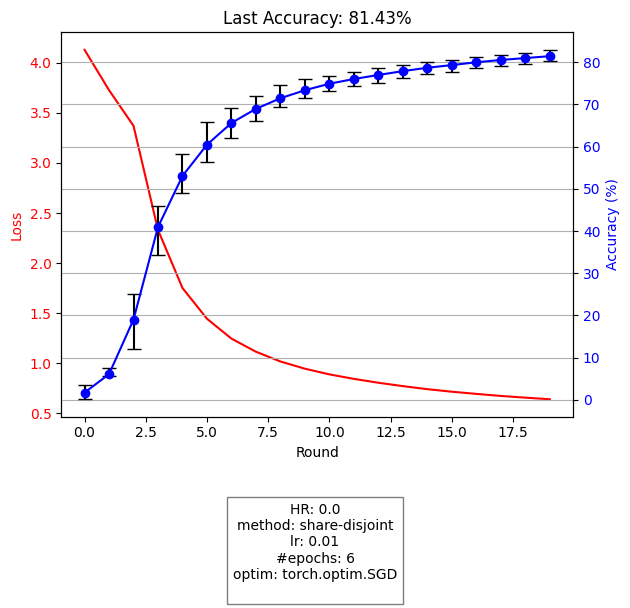
\includegraphics[width=0.8\textwidth]{../plots/femnist-horizontal/sgd/results-h0_0-hm_share-disjoint-lr0_01-e6-torch_optim_SGD.png}  % Adjust width as needed
    \caption{Caption describing the image}
    \label{fig:femnists0sgd}
\end{figure}

Un primo caso di chiara convergenza intorno all'88\% lo si vede quando 
si inizia a condividere il 20\% dei dataset come mostrato in figura 
\ref{fig:femnists2sgd}, dove si può vedere che il modello smette di 
imparare intorno al decimo round.
\begin{figure}[htbp]  % h: here, t: top, b: bottom, p: page
    \centering
    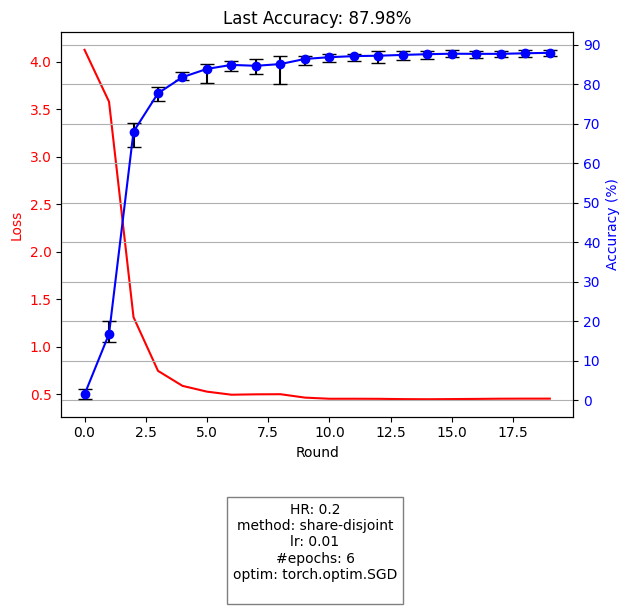
\includegraphics[width=0.8\textwidth]{../plots/femnist-horizontal/sgd/results-h0_2-hm_share-disjoint-lr0_01-e6-torch_optim_SGD.png}  % Adjust width as needed
    \caption{Caption describing the image}
    \label{fig:femnists2sgd}
\end{figure}

L'apprendimento diventa sempre più veloce e raggiunge performance 
finali migliori man mano che vengono condivisi più dati, fino all'ultimo 
esperimento fatto con un unico dataset globale condiviso, i cui risultati 
sono in figura \ref{fig:femnists9sgd}.
\begin{figure}[htbp]  % h: here, t: top, b: bottom, p: page
    \centering
    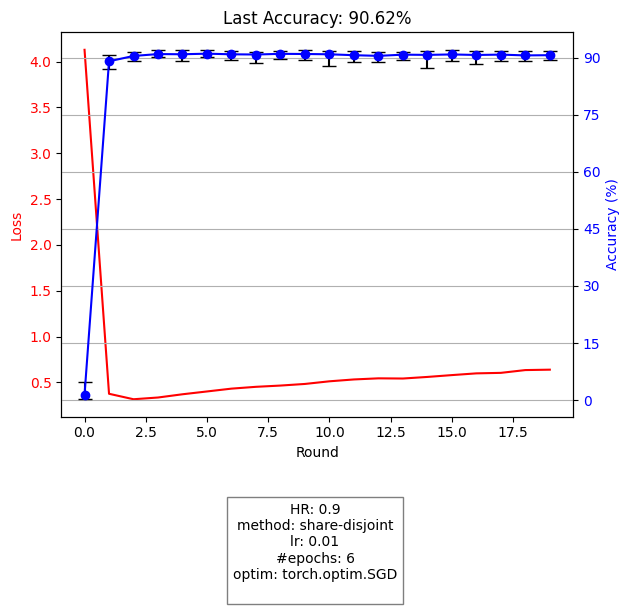
\includegraphics[width=0.8\textwidth]{../plots/femnist-horizontal/sgd/results-h0_9-hm_share-disjoint-lr0_01-e6-torch_optim_SGD.png}  % Adjust width as needed
    \caption{Caption describing the image}
    \label{fig:femnists9sgd}
\end{figure}

Dei due ottimizzatori provati, SGD è quello che performa meglio: è più 
veloce nell'apprendimento, ottiene performance migliori alla fine del 
training ed è molto più stabile. In particolare tutte le run che hanno 
utilizzato AdamW e il metodo di condivisione \texttt{unify} mostrano 
sempre intervalli di incertezza enormi, come quello riportato in 
figura \ref{fig:feministu5adam}. La situazione è analoga anche usando 
la condivisione \texttt{share-disjoint} fino a che il grado di 
condivisione non raggiunge un minimo del 30\%, come mostrato nelle 
figure \ref{fig:feminists2adam} e \ref{fig:feminists3adam}, e anche 
dopo oltre il 30\% non è garantita una maggiore stabilità, come ha 
rivelato l'esperimento con 80\% di condivisione (figura \ref{fig:feminists8adam}).
\begin{figure}[htbp]  % h: here, t: top, b: bottom, p: page
    \centering
    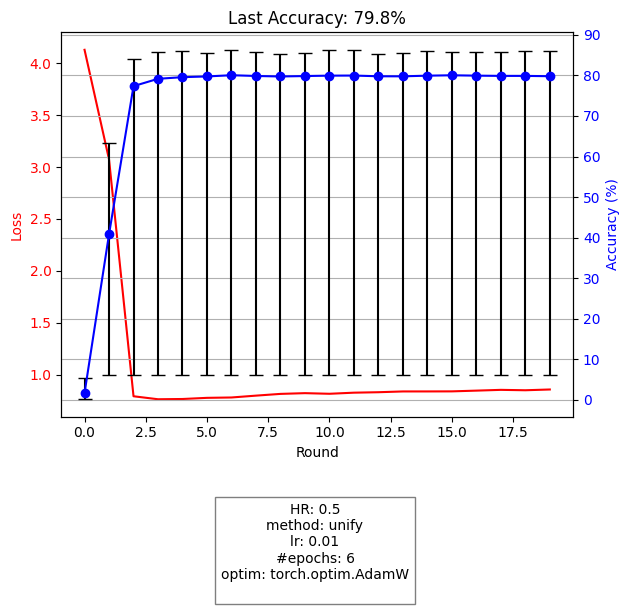
\includegraphics[width=0.8\textwidth]{../plots/femnist-horizontal/adamw/results-h0_5-hm_unify-lr0_01-e6-torch_optim_AdamW.png}  % Adjust width as needed
    \caption{Caption describing the image}
    \label{fig:feministu5adam}
\end{figure}
\begin{figure}[htbp]  % h: here, t: top, b: bottom, p: page
    \centering
    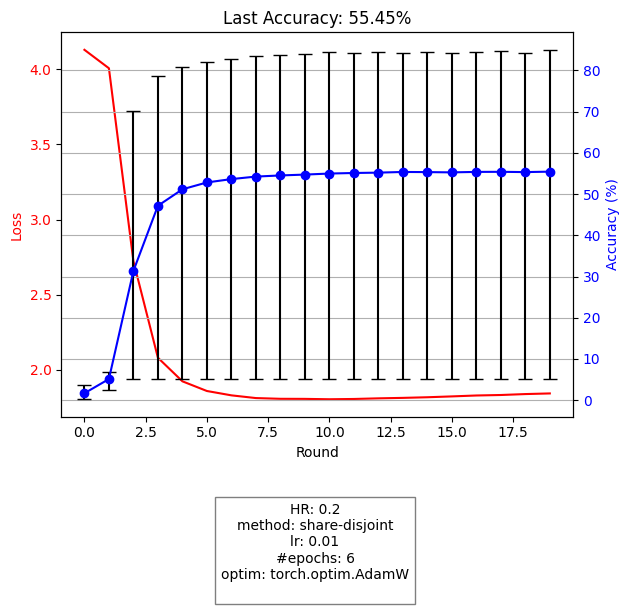
\includegraphics[width=0.8\textwidth]{../plots/femnist-horizontal/adamw/results-h0_2-hm_share-disjoint-lr0_01-e6-torch_optim_AdamW.png}  % Adjust width as needed
    \caption{Caption describing the image}
    \label{fig:feminists2adam}
\end{figure}
\begin{figure}[htbp]  % h: here, t: top, b: bottom, p: page
    \centering
    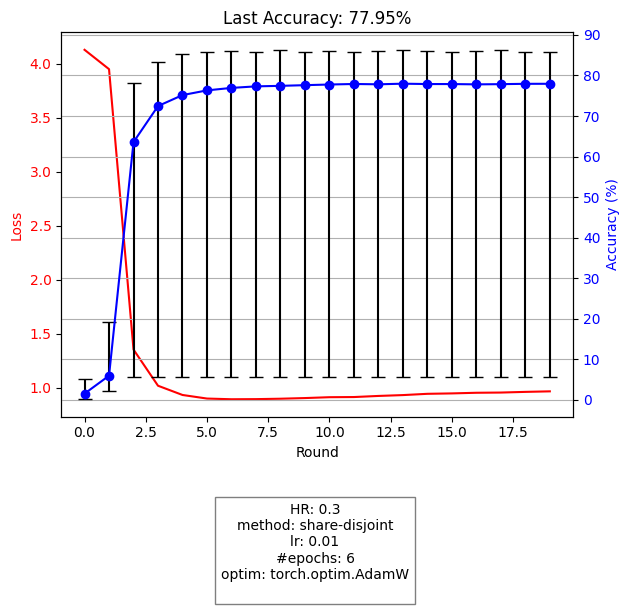
\includegraphics[width=0.8\textwidth]{../plots/femnist-horizontal/adamw/results-h0_3-hm_share-disjoint-lr0_01-e6-torch_optim_AdamW.png}  % Adjust width as needed
    \caption{Caption describing the image}
    \label{fig:feminists3adam}
\end{figure}
\begin{figure}[htbp]  % h: here, t: top, b: bottom, p: page
    \centering
    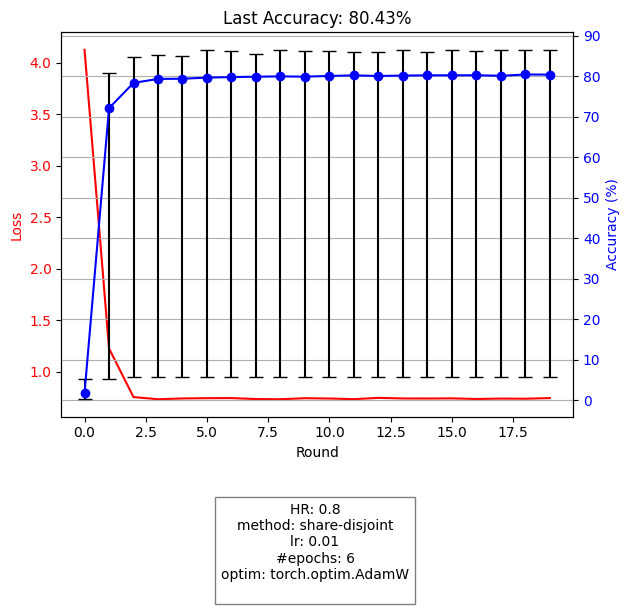
\includegraphics[width=0.8\textwidth]{../plots/femnist-horizontal/adamw/results-h0_8-hm_share-disjoint-lr0_01-e6-torch_optim_AdamW.png}  % Adjust width as needed
    \caption{Caption describing the image}
    \label{fig:feminists8adam}
\end{figure}

Guardando questi grafici si può notare come il comportamento medio non sia 
necessariamente rappresentativo di tutti i modelli allenati con AdamW, dato 
l'ampio margine d'incertezza e si potrebbe pensare che, al di là dei problemi 
di instabilità sia comunque possibile ottenere un modello performante
utilizzando quest'algoritmo. Va però notato che comunque anche i modelli 
meglio performanti allenati con AdamW, non hanno raggiunto performance 
superiori né uguali a quelle ottenute con SGD, con massimo di 90.69\%
(mediamente) per SGD, contro un 86\% circa di massimo totale.

Un'ultima osservazione che può essere fatta è come il metodo di condivisione
\texttt{share-disjoint} sia generalmente più stabile rispetto al 
\texttt{unify}. La spiegazione è semplice: \texttt{unify} scegliendo 
certi client da scegliere come dataset condivisi crea un dataset 
globale che conterrà gli stessi bias presenti nei dataset dei client 
selezionati; \texttt{share-disjoint} invece, selezionando alcuni sample 
da tutti i dataset locali, garantisce di coprire, almeno in parte, 
tutte le peculiarità nei dati di tutti i client. In questo dataset 
questo effetto non è particolarmente marcato se non con l'AdamW o nei 
primissimi round di training con basso gradi di condivisione in SGD.
\begin{figure}[htbp]  % h: here, t: top, b: bottom, p: page
    \centering
    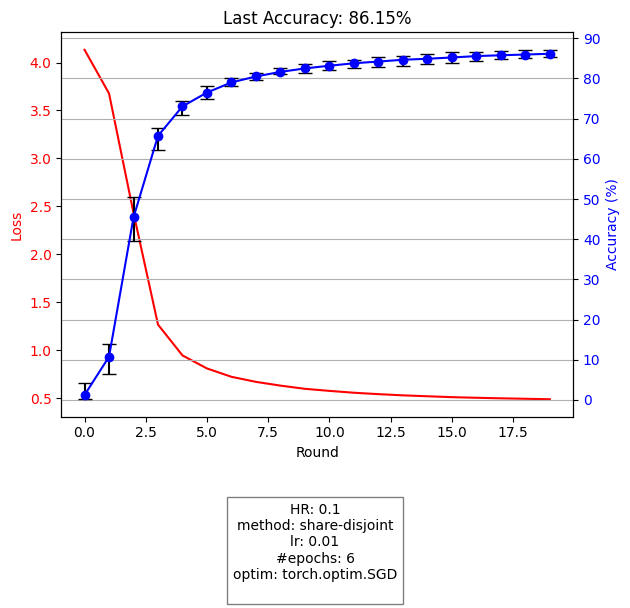
\includegraphics[width=0.8\textwidth]{../plots/femnist-horizontal/sgd/results-h0_1-hm_share-disjoint-lr0_01-e6-torch_optim_SGD.png}  % Adjust width as needed
    \caption{Caption describing the image}
    \label{fig:femnists2sgd}
\end{figure}
\begin{figure}[htbp]  % h: here, t: top, b: bottom, p: page
    \centering
    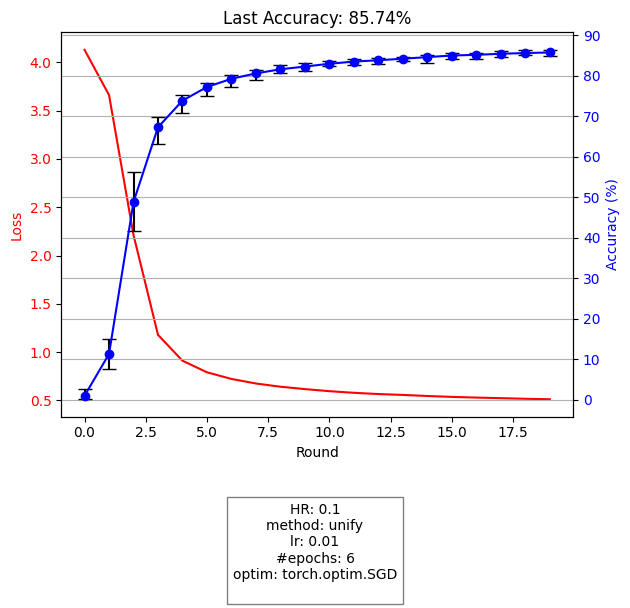
\includegraphics[width=0.8\textwidth]{../plots/femnist-horizontal/sgd/results-h0_1-hm_unify-lr0_01-e6-torch_optim_SGD.png}  % Adjust width as needed
    \caption{Caption describing the image}
    \label{fig:femnists2sgd}
\end{figure}

Quella che segue è una lista dei grafici di tutti gli esperimenti
che sono stati svolti.
TODO mettere le immagini

\section{HAR - HFL}
In questa sezione vengono descritti gli esperimenti fatti con il dataset
UCI HAR con il normale partizionamento orizzontale e vengono descritti 
i risultati.

\subsection{Set up}
Per l'UCI HAR invece è stata utilizzata una semplice MLP con un solo 
hidden layer di 50 neuroni. Di nuovo, si sono provate le 
strategie di ibridazione \texttt{unify} e \texttt{share-disjoint} con 
gradi di ibridazione da 0\% a 100\% in passi di 10\%. Anche qui sono 
stati testati sia l'ottimizzatore SGD che AdamW con learning rate 
\(\eta = 0.01\) e momentum \(\beta = 0.9\) nel caso di SGD. Il 
training ha usato 5 epoche locali, è durato 20 round e i risultati 
sono una media su 20 simulazioni consecutive. In questo caso è stato 
utilizzato l'intero dataset con 30 diversi client.

In esperimenti preliminari anche con questo dataset si è provato ad 
utilizzare SGD senza momentum e in questo caso il modello è stato in 
grado di convergere lo stesso, seppur rallentando prevedibilmente 
l'apprendimento. Sono stati provati anche valori diversi di learning 
rate come \(\eta = 0.1\) o \(\eta = 0.001\) ma non si sono viste 
differenze interessanti nell'apprendimento, se non una leggera 
instabilità maggiore o una velocità di apprendimento minore.


\subsection{Risultati}
L'UCI HAR è il dataset che ha mostrato le performance migliori.
Innanzitutto nonostante la dimensione piuttosto contenuta del modello
utilizzato si è riscuti ad avere ottime prestazioni lo stesso, non 
scendendo mai al di sotto del 90\% di accuracy e avvicinandosi al 
95\% per gli esperimenti con maggior grado di ibridazione. Le 
figure \ref{fig:hars0sgd} e \ref{fig:hars9sgd} mostrano i risultati 
ai due estremi di ibridazione.
\begin{figure}[htbp]  % h: here, t: top, b: bottom, p: page
    \centering
    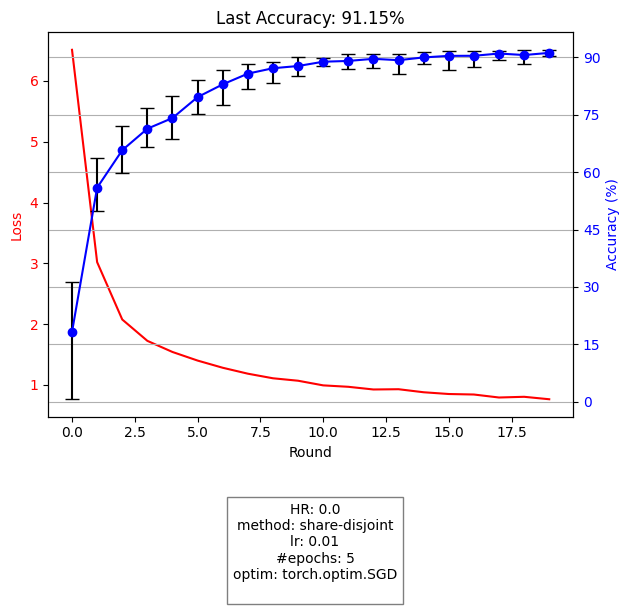
\includegraphics[width=0.8\textwidth]{../plots/har-horizontal/sgd/results-h0_0-hm_share-disjoint-lr0_01-e5-torch_optim_SGD.png}
    \caption{Caption describing the image}
    \label{fig:hars0sgd}
\end{figure}
\begin{figure}[htbp]  % h: here, t: top, b: bottom, p: page
    \centering
    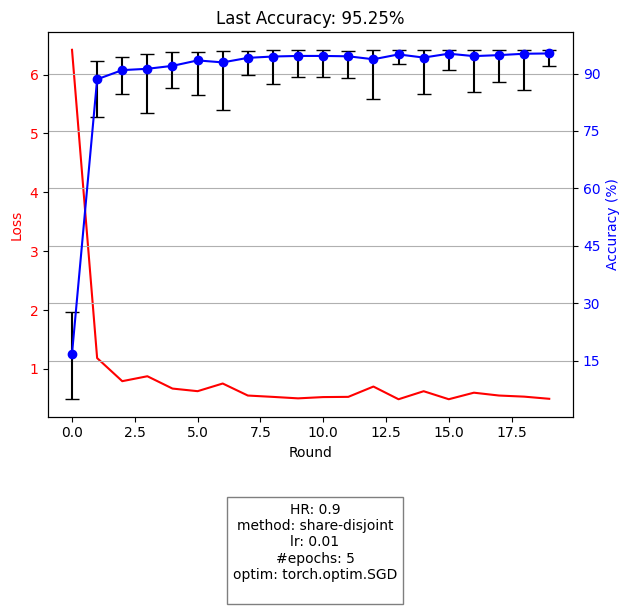
\includegraphics[width=0.8\textwidth]{../plots/har-horizontal/sgd/results-h0_9-hm_share-disjoint-lr0_01-e5-torch_optim_SGD.png}
    \caption{Caption describing the image}
    \label{fig:hars9sgd}
\end{figure}

Come si può vedere in questo caso il modello riesce ad arrivare a 
convergenza entro i 20 round di training prefissati.

Una differenza interessante rispetto al FEMNIST è che in questo 
caso AdamW si comporta sensibilmente meglio. Tanto per cominciare
le performance dei modelli allenati con SGD sono perfettamente 
comparabili a quelle dei modelli allenati con AdamW, anziché 
performare peggio. Inoltre AdamW mostra una maggiore resistenza 
all'instabilità dell'apprendimento provocata dalla condivisione 
dei dataset con il metodo \texttt{unify}. In figura 
\ref{fig:haru6sgd} si può vedere il risultato del training con SGD,
metodo \texttt{unify} al 60\% di condivisione, mentre in figura 
\ref{fig:haru6adam} si vede il risultato del training sotto le 
stesse condizioni usando l'algoritmo AdamW. Come si può vedere 
dagli intervalli di incertezza AdamW risulta più stabile in 
queste condizioni.
\begin{figure}[htbp]  % h: here, t: top, b: bottom, p: page
    \centering
    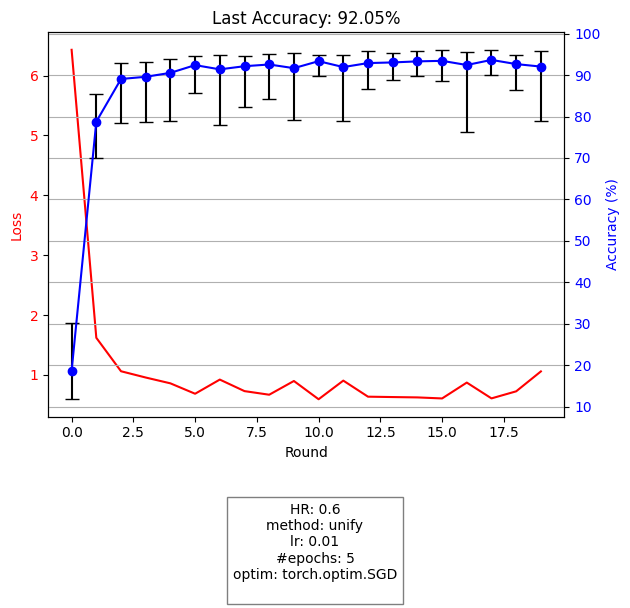
\includegraphics[width=0.8\textwidth]{../plots/har-horizontal/sgd/results-h0_6-hm_unify-lr0_01-e5-torch_optim_SGD.png}
    \caption{Caption describing the image}
    \label{fig:haru6sgd}
\end{figure}
\begin{figure}[htbp]  % h: here, t: top, b: bottom, p: page
    \centering
    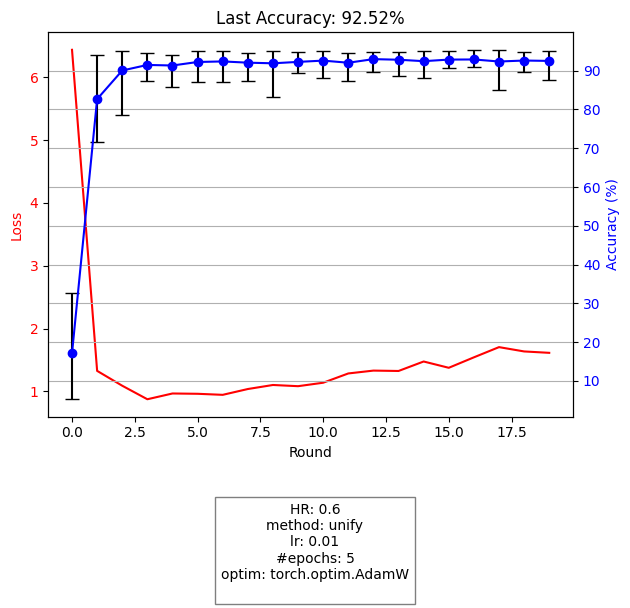
\includegraphics[width=0.8\textwidth]{../plots/har-horizontal/adam/results-h0_6-hm_unify-lr0_01-e5-torch_optim_AdamW.png}
    \caption{Caption describing the image}
    \label{fig:haru6adam}
\end{figure}

Anche per questo dataset, qui di seguito si trovano i grafici dei
risultati di tutti gli esperimenti condotti.
TODO mettere le immagini


\section{HAR - VFL}
L'ultimo esperimento fatto è quello del UCI HAR con partizionamento 
verticale delle feature.

In questo caso la rete neurale che compie la classificazione è 
distribuita tra client e server. Dato un numero di client \(K\) 
configurabile ogni ogni client ha un MLP che accetta \(561 / K\)
feature (dove l'utlimo client prende le feature rimanenti in caso di 
resto diverso da 0) e ne calcola un encoding. Sono state provate due 
dimensioni diverse di encoding: su un vettore lungo 10 e lungo 100.
Data la lunghezza \(l\) del vettore di encoding, il server ha un'altra 
MLP che accetta un vettore lungo \(Kl\) e ne calcola la classificazione.
Sia il modello dei client che quello del server hanno un hidden layer 
di 50 neuroni.

I risultati di questo esperimento sono stati però deludenti: a discapito
di quale ottimizzatore venisse utilizzato tra SGD e AdamW, del numero di client da 
3 a 50 e della dimensione dell'encoding non si è mai riusciti ad ottenere 
un'accuracy superiore al 18\%, rimanendo quindi appena sopra
1 / 6 = 16.7\% cioè la probabilità di prenderci tirando a caso ogni 
volta su 6 classi. Si può quindi concludere che questo partizionamento
delle feature su questo dataset non è un approccio funzionante.